\begin{figure}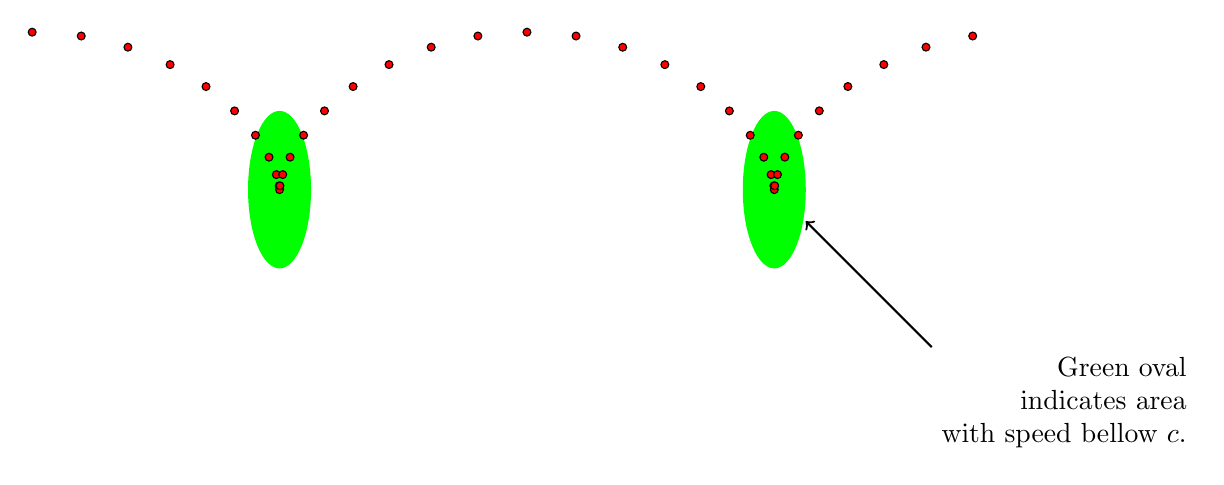
\begin{tikzpicture}[scale=1, rotate=0]

% single ornac of a photon  going through two cycloid cycle in red
% with green oval to indicate the under c area

% greeen oval
\path
(pi,0) node (bottom1){}
(3*pi,0) node (bottom2){};
\draw [draw = none, fill = green]
 (bottom1) circle [ x radius = 0.4, y radius = 1 ]
 (bottom2) circle [ x radius = 0.4, y radius = 1 ]node (greenoval) {};

\draw[<-, thick] (greenoval)+(0.4,-0.4) -- ++(2,-2) node (slowspeed){}; 
\path
(slowspeed) node [below right , align=right]
{Green oval \\ indicates area \\ with  speed bellow $c$.};


%% red ornac
 \foreach \x in {0, 0.05,...,2}
  {
    \draw[black, fill=red] 
   ({((2*pi*\x + sin(2*pi*\x r)) },{1 + cos(2*pi*\x r) }) circle [radius=0.05];
  }


\end{tikzpicture}\caption{Single ornac of a photon  going through two cycloid cycle in red
 with green oval to indicate the under c area
\label{fig:photon_red_ornac_green_area}}
\end{figure}
